\chapter{Introduction}

\textit{Rendering} is generally the process of generating a 2-dimensional image, called \textit{render}, from the mathematical description of a 3-dimensional scene. 
%To oversimplify it, a scene is made of light sources, geometries and a camera, all defined in mathematical, hence rather abstract, terms. 
Several rendering algorithms have been developed over the years and many of them have been designed to produce images as \textit{photorealistic} and lifelike as possible. The most recent ones of these kind are all based upon simulating how light interacts with the scene, closely imitating its natural behavior. A particularly successful rendering algorithm following this philosophy is \textit{Path Tracing} \cite{kajiya1986rendering} since its derivation and itself are widespread across animation, visual effects and video games. In simple words, path tracing is based upon the idea of shooting rays out of an artificial camera towards the scene and make each bounce around the scene until it reaches a light source; then, the luminous energy carried by the ray and its bounces, called \textit{path}, can be computed --- or \textit{traced} back. Without even diving into its details --- which are left for section \ref{background} ---, it is clear how complex path tracing can get. This makes it difficult to grasp by people approaching it and difficult to debug.

We are presenting a tool capable to show the user an overview of the inner workings of a path tracer by providing interactive visualizations of the very core of a path tracer: paths and how they interact with the scene.
We strived to create something that does not tell but --- literally --- shows the swarm of paths shot by a path tracer to help understand what is actually going on during the rendering process.

The idea of providing interactive renderings of the data generated by a path tracer --- or a ray tracer --- is not original. Let us mention a few that inspired our work:
\begin{itemize}
	\item The \textit{Ray tracing visualization toolkit} by C. Gribble et Al. \cite{gribble2012ray} is nice starting point but it only focuses on single rays, hence it does not show how multiple paths behave. We believe that analyzing just one path at once is not enough to grasp the entities involved. A more global view is crucial.
	\item The work presented in \textit{A Framework for Visual Dynamic Analysis of Ray Tracing Algorithms} by H. Lesev and A. Penev \cite{lesev2014framework} has amazing filtering and data gathering features which inspired us, but it dwells on the idea of debugging and analyze data generated by ray tracers \cite{whitted1979improved}\cite{cook1984distributed} while we focused especially on path tracing.
	\item Another great inspiration for us was the framework presented in \textit{Applying Visual Analytics to Physically Based Rendering} by G. Simons et Al. \cite{simons2019applying}, especially the visualization parts. We however drift off it because, while they reduce the data they gather from a path tracer by selecting only about 1/6000th of the total paths, our goal is to keep the whole dataset and let the user choose what to visualize from all the samples.
	\item Another tightly related work is \textit{EMCA}, which stands for \textit{Explorer of Monte-Carlo based Algorithms}, by C. Kreisl \cite{EMCA@2019}. It focuses on path tracing and visualizations but its client-server architecture with per-pixel path analysis lacks of the global view we are trying to achieve.
\end{itemize}  

\section{Background}
\label{background}

To fully comprehend the topics and challenges presented in this work a background is needed.

\subsection{The rendering equation}
\textit{Photorealistic rendering} is the process that given a mathematical description of a 3-dimensional scene outputs an as life-like as possible image, know as \textit{render}. The process simulates how light travels from light sources to a --- abstract --- camera sensor while interacting with the scene.

\subsection{Monte Carlo integration}

\subsection{Path tracing}

\subsection{OpenGL}

%It means that the algorithms that generated these datasets have different ways of choosing the direction of each path bounce in order to maximize the radiance carried by each path, speeding up the convergence of the Monte Carlo integration and hence trying to lower the amount of noise given the same amount of pixel samples. This technique, used in every application of Monte Carlo methods, is called \textit{importance sampling} \cite{kalos2009monte}. Multiple importance sampling \cite{veach1995optimally}.

\section{Motivation}
\label{motivation}
%As introduced above, path tracing is an algorithm that is not easy to picture. For someone who got to understand it, the rendering equation is more than enough to tell how a path tracer work. At least to get started, everything a person needs to know is in that equation: once combined with Monte Carlo integration, everyone is theoretically ready to implement a path tracer. 

As introduced above, path tracing is not easy to picture. This is true for both the newbie trying to implement one for the first time and the expert trying to debug a nasty case. As many research groups before us thought, having a tool showing what a tracer is doing by visualizing its interactions with the 3d scene would be grand since it would help the professional developers and the students alike. The challenge this vision has to face is the bigness, in terms of size, of these interactions. Talking about path tracing, to have a decent render, more than two hundreds paths have to be shot for each pixel: to produce an image, more than fifty million paths have to be shot. Postponing data size considerations for later (ref. \ref{datatogather}), leaves us with potential datasets that without proper data reduction or filtering are of no use to anyone. Related works usually perform substantial reductions of the datasets \cite{simons2019applying}\cite{EMCA@2019}, but we believe that having all the paths available to visualization would improve the experience.

With these premises, a more precise idea for a visualization tool came to us. 
The user should have the power to visually and interactively explore all the paths previously generated by a path tracer during rendering. The paths have to be immersed in an interactive rendering of the scene: their most important property is their geometry or, in other words, where they bounce inside the scene. Even if out of curiosity and naivety we tried visualizing all the paths of smaller datasets achieving compelling yet disastrously cluttered results (fig. \ref{visual_clutter}), visualizing the millions of paths all together was out of question since the beginning. To navigate this ocean of paths, the user should be provided with a global summary overview of the dataset in its entirety, and they should also able to filter them using spatial queries. For the global overview we envisioned a heatmap applied as a texture to the 3d view of the scene that shows areas where there is more path activity, while for the spatial queries we thought the user might want to select path bouncing on certain noteworthy surfaces, such as lights or mirrors. 

\begin{figure}
	\centering
	\centering
	\begin{subfigure}[t]{0.49\linewidth}
		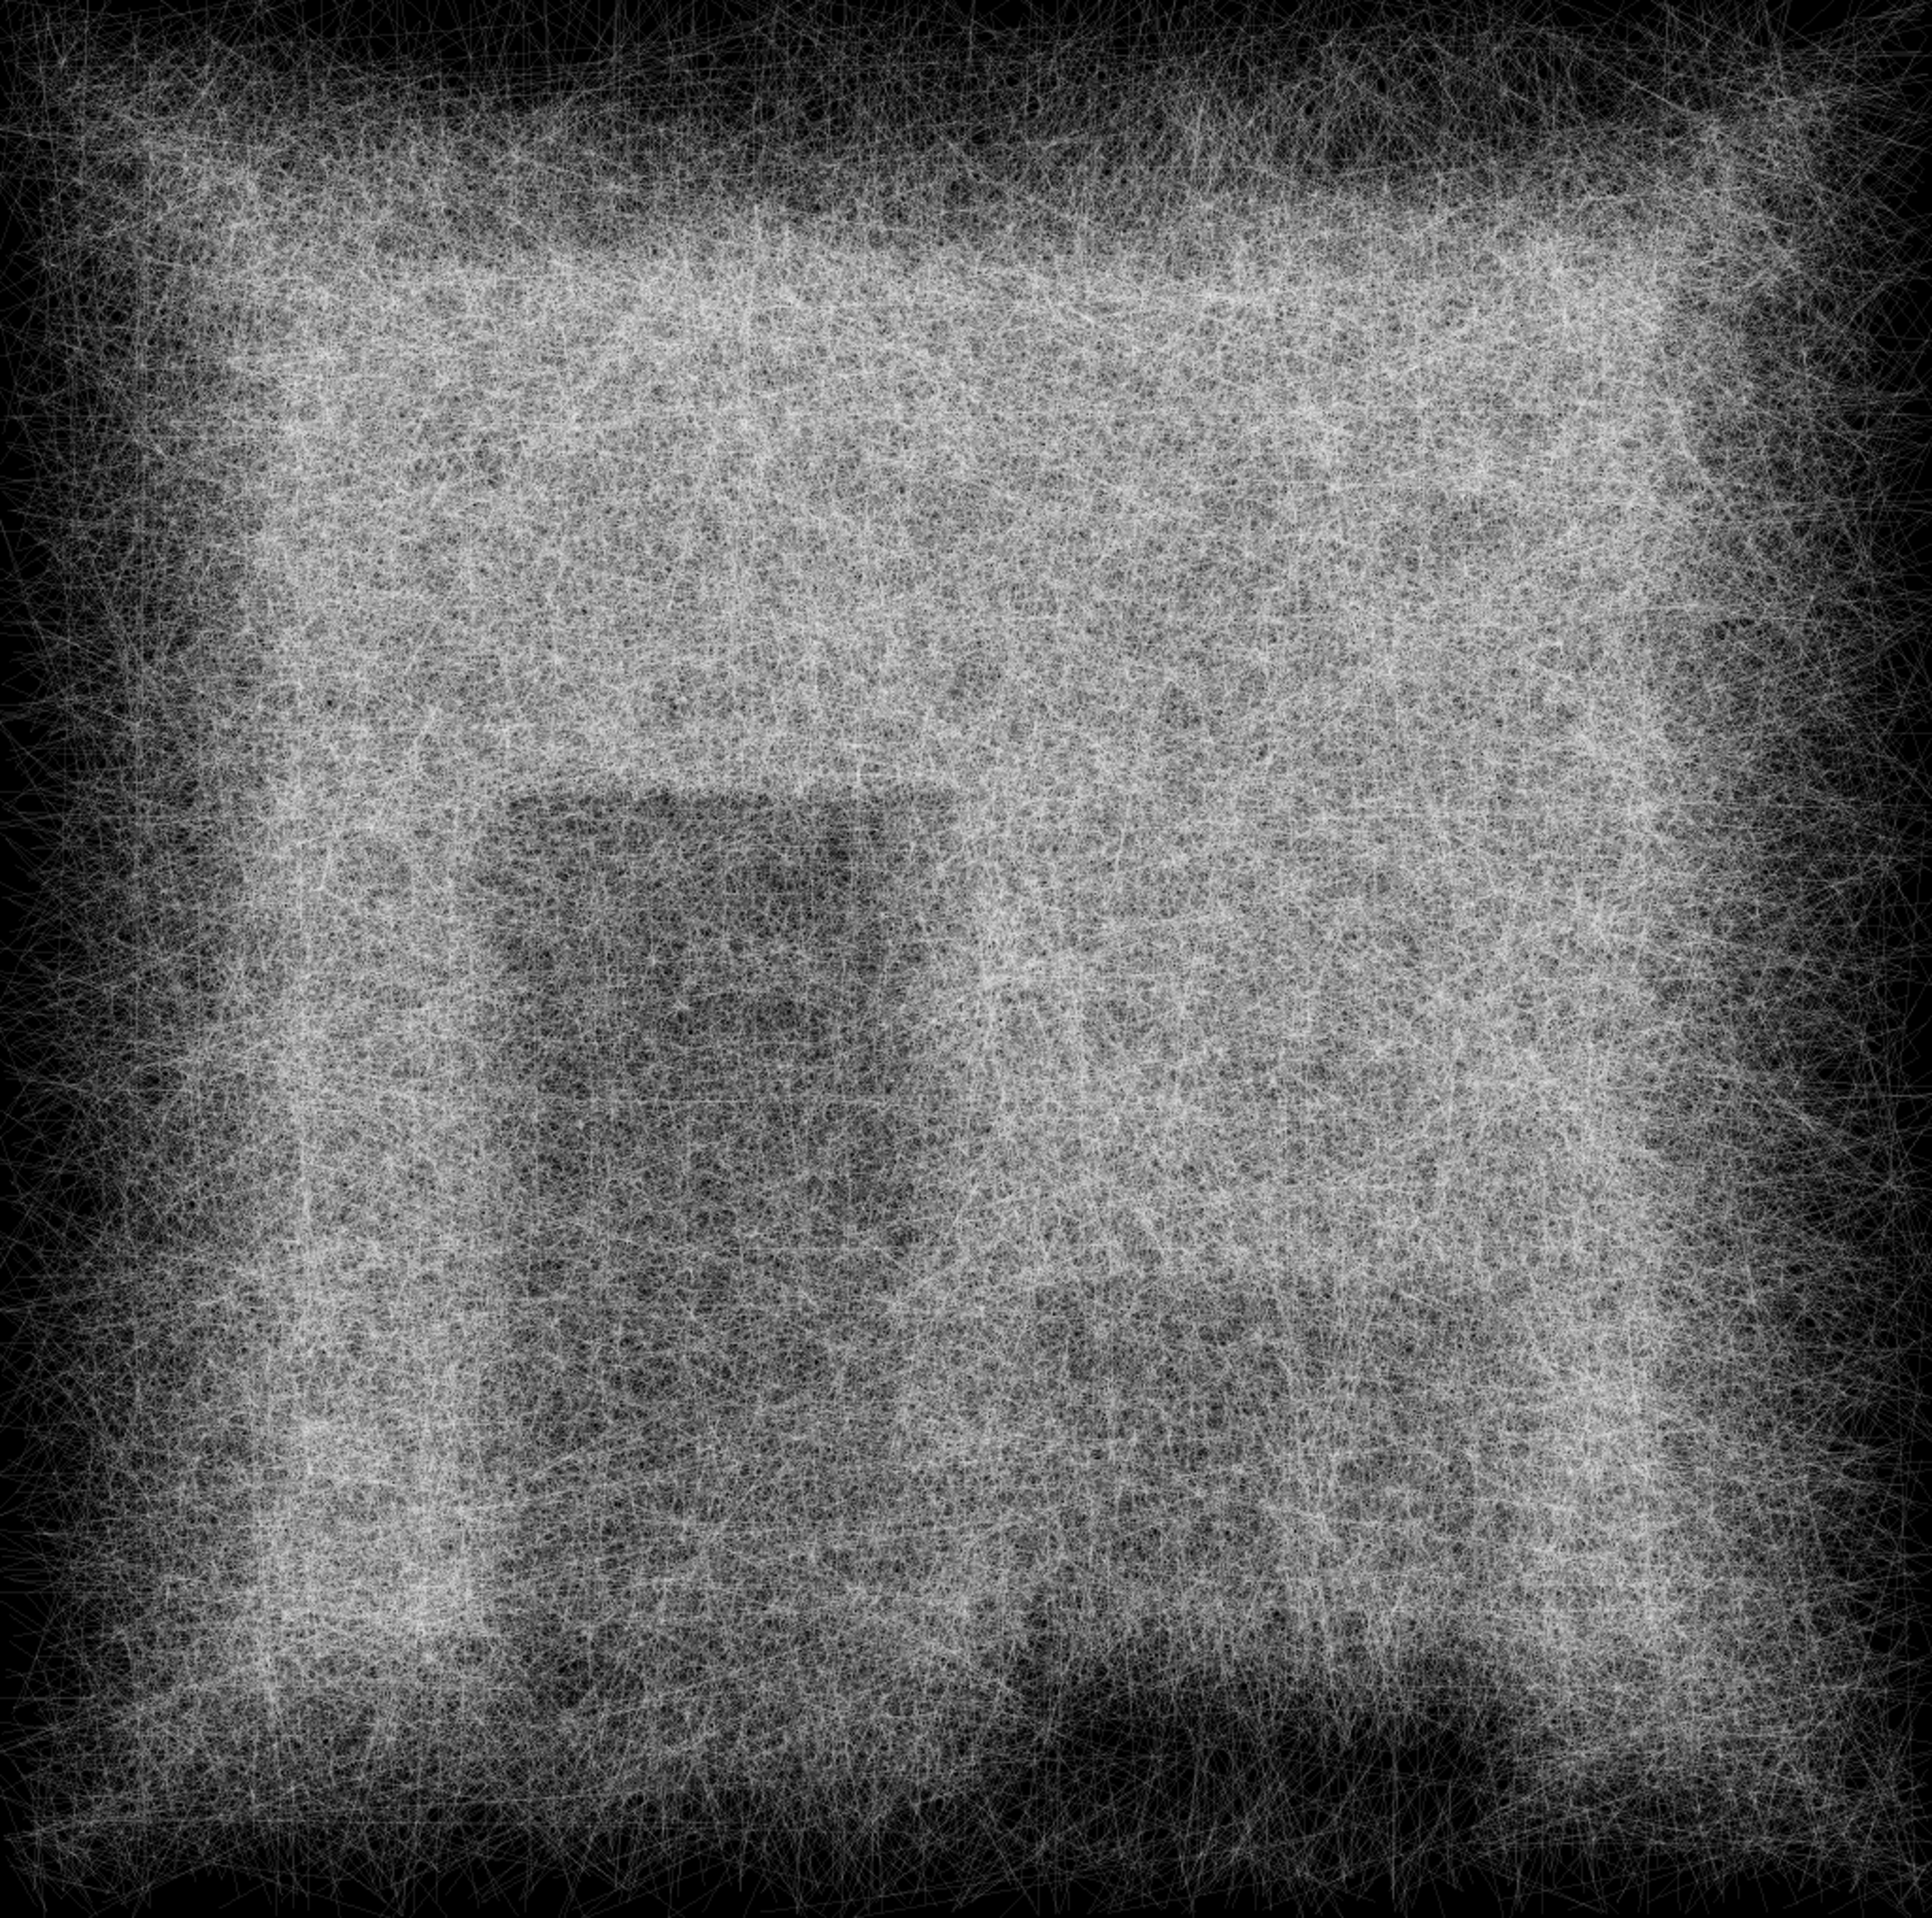
\includegraphics[width=\textwidth]{chapters/chapter_intro/clutter_early1}
		\caption{$64 \times 64$, 1 spp}
	\end{subfigure}
	\begin{subfigure}[t]{0.49\linewidth}
		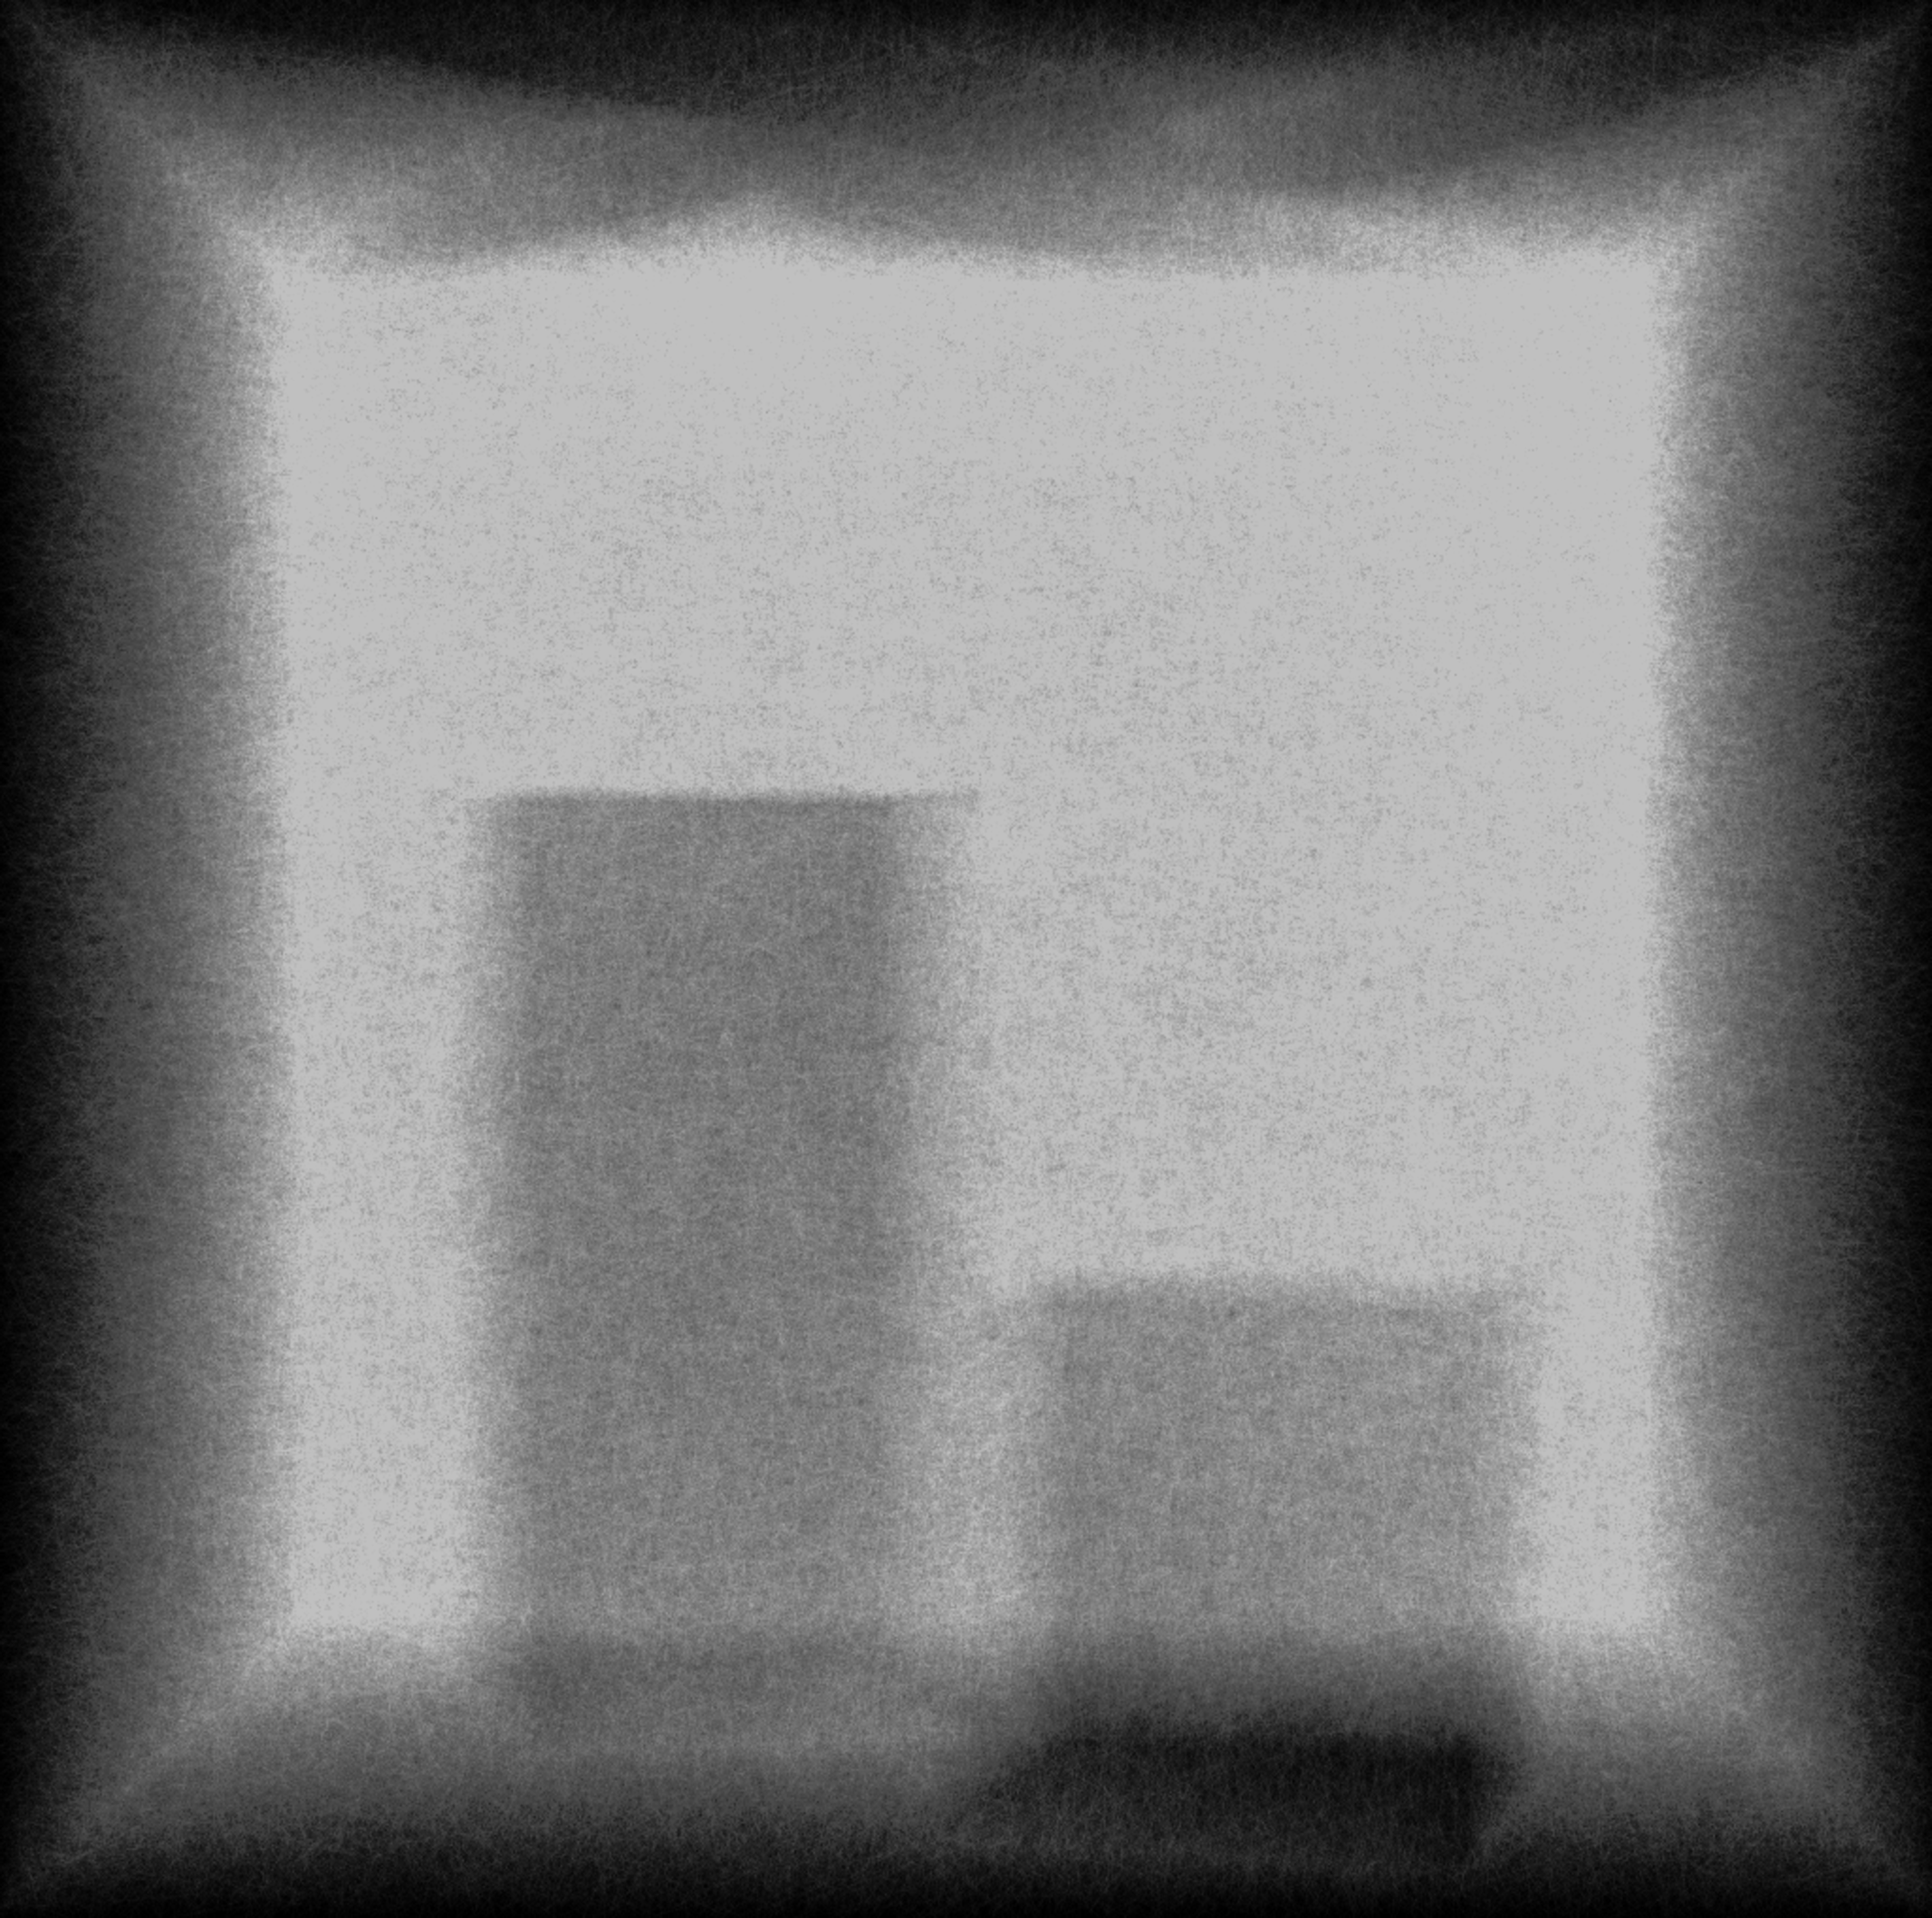
\includegraphics[width=\textwidth]{chapters/chapter_intro/clutter_early2}
		\caption{$64 \times 64$, 64 spp}
	\end{subfigure}
	
	\caption{Visual clutter in an early version of the tool where the scene rendering has not been implemented yet. Both datasets have been generated on the \textit{Cornell Box} scene.}
	\label{visual_clutter}
\end{figure}

Later in the development, it became clear that the possibility of comparing different datasets would come in handy to users. It could be useful in many cases such as comparing two progressive versions of the same in-development path tracer to understand what changed or, more in an educational context, such as showing a ground truth next to a purposely wrong dataset to understand why one is wrong on a deeper level.

Of course, before even talking about visualizing data, data has to be gathered from a path tracer. We envisioned a software piece, parallel to the visualization client, able to plug to any path tracer and gather with little effort the required data during the rendering process. Then the idea of a gathering library with a very simple interface came about; a library that can be plugged into any path tracer the user is currently working on by just calling the few required functions.

To summarize, our vision consisted in a tool divided into a visualization client and a data gathering library which can be used both for debugging and teaching purposes. The library should have an easy to interact with interface, while the client would let the user explore different datasets simultaneously and in their entirety using the filtering and visualization options provided to them.

%select a portion of a surface of the 3d scene the tracer has been run upon and see the paths that bounce there with a bunch of useful data. To be able to do that the whole set of paths shoot by a tracer are needed: by the very stochastic nature of a path tracer, it is impossible to determine which paths will end up bouncing where without resolving them all first. That is why it has been decided it was essential to store data about each path during the rendering process. To make the tool usable in most possible use cases, it had to be able to plug into an existing path tracer and this lead to the conception of the tool as a two software pieces suite: a \textit{data gatherer library} called \texttt{gatherer} and a \textit{visualization client} called \texttt{gathererclient}.

%Now this “useful data” was not extremely well-defined during those early stages, so most of the efforts have been directed to the very essential: rendering the requested paths keeping interactivity.